\documentclass[conference]{IEEEtran}
\IEEEoverridecommandlockouts
% Template version as of 6/27/2024
\usepackage{cite}
\usepackage{amsmath,amssymb,amsfonts}
\usepackage{algorithmic}
\usepackage{graphicx}
\usepackage{textcomp}
\usepackage{xcolor}
\def\BibTeX{{\rm B\kern-.05em{\sc i\kern-.025em b}\kern-.08em
    T\kern-.1667em\lower.7ex\hbox{E}\kern-.125emX}}
\begin{document}

\title{FRESCA-Net: A Compact From-Scratch Convolutional Network with Energy-Domain Between-Class Learning for Environmental Sound Classification}

\author{\IEEEauthorblockN{Anonymous Author(s)}
\IEEEauthorblockA{\textit{Affiliation and contact details} \\
\textit{withheld for double-blind review}}
}

\maketitle

\begin{abstract}
Environmental sound classification is a core capability for acoustic monitoring, surveillance and bioacoustic sensing, yet the field-standard ESC-50 benchmark remains hard because it offers only two thousand clips spread across fifty classes. Recent leaderboard progress is dominated by large transformers pretrained on external audio corpora, which reach ninety-five to ninety-eight percent accuracy but are unusable when no external data, no pretraining and a small on-device budget are the operating constraints. This work proposes FRESCA-Net, a compact 2.88 M-parameter residual network trained entirely from scratch on ESC-50, and benchmarks it against the published from-scratch family under one leakage-free protocol. FRESCA-Net couples a squeeze-and-excitation residual backbone with a frequency-coordinate channel, anisotropic downsampling that keeps a genuine temporal sequence, and an attentive-statistics pooling head; its main data lever is an energy-domain Between-Class mixing applied to the raw waveform before the mel transform, so that the mixing stays energy-additive. Under the official five-fold cross-validation and a fixed-budget, stochastic-weight-averaged evaluation without any checkpoint selection on the test fold, a single FRESCA-Net reaches 81.55 percent accuracy and a three-seed ensemble reaches 82.45 percent, exceeding human accuracy (81.3 percent) and matching EnvNet-v2 with Between-Class learning (81.8 percent). A matched ablation attributes 16.45 points to the architecture and 2.90 points to the augmentation, and shows that a 300-epoch budget overfits the sixteen-hundred-clip folds. FRESCA-Net therefore provides a reproducible, leakage-free reference for compact from-scratch environmental sound recognition.
\end{abstract}

\begin{IEEEkeywords}
environmental sound classification; ESC-50; convolutional neural networks; between-class learning; squeeze-and-excitation; attentive pooling; from-scratch training; edge audio
\end{IEEEkeywords}

\section{Introduction}
Automatically naming the sounds around us --- a dog barking, a chainsaw, rain, a crying baby --- underpins acoustic surveillance, urban noise monitoring, smart-home context sensing and bioacoustic ecology, yet a human annotator quickly becomes the bottleneck on any large or continuous stream of audio. The ESC-50 dataset \cite{piczak_dataset} has become the reference benchmark for this problem: fifty everyday sound categories, forty clips each, arranged into five predefined folds for cross-validation. Its very compactness is what makes it hard. With only two thousand five-second clips over fifty classes, a model sees roughly sixteen hundred training clips per fold and is exposed to overfitting in a way that large speech and music corpora are not; the hand-crafted baselines that accompanied the dataset reached only 44.3, 39.6 and 32.2 percent \cite{piczak_dataset}.

Convolutional neural networks quickly became the workhorse of the benchmark. A shallow two-convolution network on mel-spectrograms with a tall vertical first-layer filter already lifted accuracy to 64.5 percent \cite{piczak_cnn}, and pairing a deeper convolutional network with audio-specific data augmentation such as time-stretching and pitch-shifting pushed it further \cite{salamon_bello}. A second line of work moved the input closer to the signal, learning directly from the raw waveform with an end-to-end network \cite{tokozume_envnet} and with very deep one-dimensional stacks \cite{dai_rawwaveform}, while a parallel strand asked how much the choice of time--frequency representation itself matters for a fixed convolutional stack \cite{huzaifah_tf}. Because the labelled data is so scarce, regularisation and augmentation carry an unusually large share of the accuracy. Between-Class learning, which mixes two training examples in a proportion and asks the network to predict the mixing ratio, proved to be a particularly strong lever on environmental audio \cite{tokozume_bc}; multi-scale convolutions that fuse waveform and spectrogram views added complementary gains \cite{zhu_multiscale}; and transferring representations learned from the audio track of unlabelled video gave a strong starting point for the smallest supervised sets \cite{aytar_soundnet}.

The most recent and highest numbers on ESC-50, however, come from a fundamentally different regime. Large convolutional and transformer backbones trained on the AudioSet corpus of over two million weakly labelled clips \cite{hershey_cnnaudio}, \cite{gemmeke_audioset}, and their descendants --- the pretrained audio neural networks of \cite{kong_panns}, the audio spectrogram transformer \cite{gong_ast}, the self-supervised acoustic tokeniser of \cite{chen_beats} and the language-audio contrastive model of \cite{elizalde_clap} --- now report ninety-five to ninety-eight percent on ESC-50. These results are impressive but they are not comparable to a model that must be trained on the two thousand ESC-50 clips alone: they carry hundreds of hours of external supervision into the task. The same caveat applies to cross-domain transfer that borrows an ImageNet-pretrained image backbone for spectrograms \cite{guzhov_esresnet}. When the external data, the pretraining budget and, ultimately, the parameter and latency budget of an edge device are all removed, the honest question becomes how far a compact network trained from scratch can go, and here the published numbers are both lower and, more troublingly, scattered across protocols that do not always agree on how the held-out fold is used \cite{palanisamy_rethinking}.

This study addresses that gap. We propose FRESCA-Net, a compact residual network of 2.88 million parameters trained end-to-end on ESC-50 with no external data and no pretraining, and evaluate it against the published from-scratch family under a single, deliberately leakage-free five-fold protocol: rather than selecting the best epoch on the very fold being tested --- a subtle but common source of optimism --- we fix the training budget in advance and report a stochastic-weight-averaged model, so every clip is scored once by a model that never saw its fold. On top of the architecture we run a matched two-by-two ablation that separates the contribution of the network from that of the augmentation, and a small multi-seed ensemble to probe the ceiling of the regime. The contribution is threefold: a compact architecture that reaches human-level accuracy on ESC-50 from scratch, a clean protocol and ablation that decompose architecture from augmentation, and a reproducible reference point for compact environmental sound recognition where external data is unavailable.

\section{Materials and Methods}

\subsection{Dataset and Evaluation Protocol}
We use the ESC-50 dataset \cite{piczak_dataset} exactly as published: 2000 single-channel clips of five seconds sampled at 44.1 kHz, fifty balanced classes of forty clips, and the five author-defined folds. All experiments follow the official five-fold cross-validation --- for a held-out fold $k$ the model is trained on the other four folds and tested on $k$ --- so that each clip is tested exactly once and the mean over the five folds is a leave-one-fold-out estimate over the whole dataset. Because the classes are balanced, we report classification accuracy per fold and its mean and standard deviation across folds. Fig.~\ref{fig:data} shows how varied and unforgiving the raw material is: an impulsive dog bark, stationary rain, a harmonically rich crying baby and a periodic clock tick occupy completely different regions of the time--frequency plane, and the network has to separate all fifty such classes from only sixteen hundred training clips.

\begin{figure*}[t]
\centerline{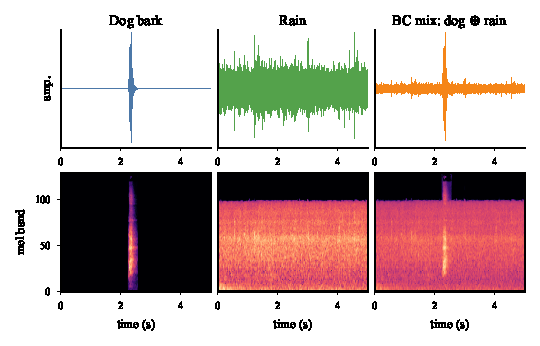
\includegraphics[width=\textwidth]{fig_dataset.pdf}}
\caption{Raw waveforms (top) and the 128-band log-mel spectrograms that FRESCA-Net actually consumes (bottom) for four ESC-50 classes and, at right, an energy-domain Between-Class mixture of the dog and rain clips computed on the raw waveform exactly as in training. The mixture overlays the impulsive bark onto the broadband rain while preserving total energy, which is the augmentation signal the network learns to disentangle.}
\label{fig:data}
\end{figure*}

We are explicit about the evaluation being leakage-free, since the small folds make it easy to be optimistic. No early stopping, checkpoint selection or exponential-moving-average selection is ever performed on the test fold. Instead the training budget is fixed in advance at 200 epochs, and the headline number is the stochastic-weight-averaged model \cite{izmailov_swa} formed from the last thirty epochs, with its batch-normalisation statistics recomputed on the training folds only. At inference we average the softmax outputs of three evenly spaced crops of the clip, a label-free test-time augmentation that is standard for ESC-50. Pretrained transformers that use external corpora are outside this comparison and are cited only for orientation.

\subsection{On-GPU Log-Mel Front-End}
The front-end computes a log-mel spectrogram on the GPU with a 1024-point short-time Fourier transform, a 512-sample hop and 128 mel bands, followed by a logarithm. Each spectrogram is standardised per instance to zero mean and unit variance; this is deliberately a per-clip statistic so that no train/test normalisation constant is ever shared, and it also makes the representation robust to the energy shift introduced by the mixing described below. Because a mel axis is not translation-invariant --- a pattern shifted up in frequency is a different sound, not the same sound moved --- we append a fixed frequency-coordinate channel to the log-mel input, following the CoordConv idea of giving a convolution explicit access to its position \cite{liu_coordconv}. The network input is therefore a two-channel image of the standardised log-mel and its coordinate map. The whole transform is parameter-free, which is what allows the augmentation to act on the raw waveform before the transform and still be seen by the network as a normal spectrogram.

\subsection{Waveform Augmentation and Energy-Domain Between-Class Learning}\label{sec:aug}
The strongest regulariser in the sixteen-hundred-clip regime is a random three-second crop of the five-second clip at training time, matched at test time by the three-crop averaging above. On top of the crop we apply mild waveform perturbations --- a circular time shift, a random gain and additive noise at a controlled signal-to-noise ratio --- and, on the spectrogram, a short-ramped SpecAugment that masks a few frequency and time bands \cite{park_specaugment}.

The principal data lever is Between-Class learning \cite{tokozume_bc}. Two root-mean-square-normalised waveforms $x_1$ and $x_2$ are mixed with a per-sample ratio $p$ drawn uniformly, and the target becomes the same convex combination of their one-hot labels,
\begin{equation}
x = \frac{p\,x_1 + (1-p)\,x_2}{\sqrt{p^2 + (1-p)^2}}, \label{eq:bc}
\end{equation}
where the denominator preserves the energy of the mixture. This is deliberately performed on the raw waveform, before the short-time Fourier transform, because sound energy is additive in the waveform domain; mixing already-computed log-mel images would break that energy-additive semantics and change what the mixing ratio means. Between-Class learning is related to the more general mixup \cite{zhang_mixup} but is specialised to the physics of the acoustic signal. When mixing is active we train the soft targets with a cross-entropy against the mixed label; label smoothing \cite{muller_labelsmoothing} is used only on the batches where mixing is off, so that the two never compound.

\subsection{The FRESCA-Net Architecture}
FRESCA-Net --- for \emph{Frequency-aware Residual Squeeze-Excitation with energy-aware between-Class and Attentive pooling} --- is a squeeze-and-excitation residual network built for the small-data, single-GPU regime. The backbone is an eighteen-layer residual network in the sense of \cite{he_resnet}, with every basic block recalibrated by a squeeze-and-excitation channel-attention unit \cite{hu_senet} and regularised on its residual branch by stochastic depth \cite{huang_stochastic}. Two design choices adapt the generic backbone to spectrograms. First, the downsampling is anisotropic: after an initial isotropic reduction the two deeper stages stride only along frequency, collapsing the frequency axis by a factor of sixteen while dividing the time axis by only four, so that a genuine temporal sequence of about sixty-five frames survives to the top of the network. Second, that surviving sequence is summarised not by a global average but by an attentive-statistics pooling head \cite{okabe_asp}, which learns a per-frame attention weight and returns both the attention-weighted mean and standard deviation over time; this preserves the temporal salience that global pooling discards, which matters for transient events such as a glass break or a dog bark. The complementary idea of factorising a block into a two-dimensional frequency path and a broadcast one-dimensional temporal path \cite{kim_bcresnet} informed the anisotropic design. Fig.~\ref{fig:arch} details the complete architecture --- from the on-GPU front-end through the four residual stages to the attentive-statistics head, with the internal wiring of one SE basic block --- and annotates the tensor shape after every stage at the three-second training crop; the whole network holds 2.88 million trainable parameters. As a controlled, apples-to-apples baseline we retrain the classic Piczak convolutional network \cite{piczak_cnn} under the identical pipeline; its published 64.5 percent gives a familiar anchor.

\begin{figure*}[t]
\centerline{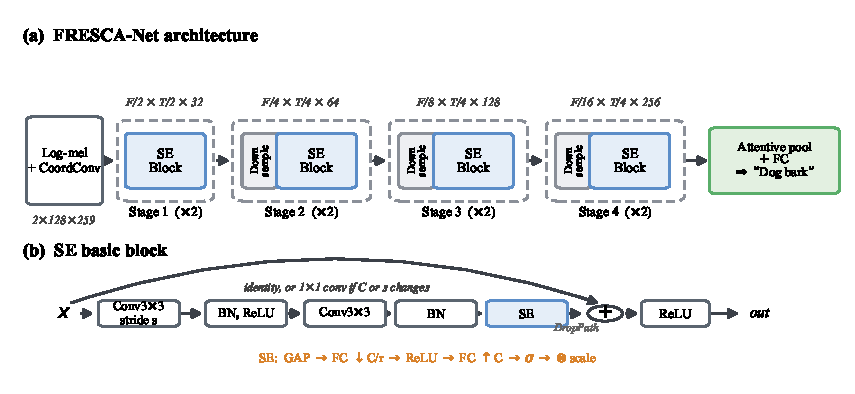
\includegraphics[width=\textwidth]{fig_arch.pdf}}
\caption{FRESCA-Net architecture. (a) A standardised log-mel spectrogram with an appended CoordConv frequency channel enters a stem and four stages of two SE basic blocks each; the two deepest stages stride only along frequency (anisotropic downsampling), as the on-top shapes show --- the frequency axis $F$ is divided by up to sixteen while the time axis $T$ is divided by only four, so a real temporal sequence survives to the attentive-statistics pooling head before the classifier. (b) One SE basic block: two $3\times3$ convolutions, squeeze-excitation channel recalibration, and a stochastic-depth residual added to an identity (or $1\times1$-conv) shortcut. The on-GPU front-end and energy-domain Between-Class augmentation that produce the input are described in Section~\ref{sec:aug} and Fig.~\ref{fig:data}.}
\label{fig:arch}
\end{figure*}

\subsection{Training Protocol}
Every model is trained end-to-end with the AdamW optimiser \cite{loshchilov_adamw} at a $1\times10^{-3}$ learning rate and $5\times10^{-4}$ weight decay, with batch normalisation and bias parameters excluded from decay. The schedule is a one-epoch linear warm-up followed by cosine annealing \cite{loshchilov_sgdr} down to $1\times10^{-5}$, over the fixed 200-epoch budget, with a batch size of 64 and mixed-precision training on a single CUDA GPU; batch normalisation \cite{ioffe_bn} stabilises the deeper stages. The last thirty epochs feed the stochastic weight average \cite{izmailov_swa} that forms the reported model. This single recipe is applied unchanged to every architecture and every ablation cell, so that differences in the tables are attributable to the factor under study and not to per-model tuning. We stress, as a matter of fairness, that a shared recipe isolates a factor at a fixed cost but does not show any single model at its own optimum; per-architecture tuning is left to future work. To push the ceiling of the from-scratch regime we additionally train a three-seed ensemble, in which for each held-out fold three FRESCA-Net models with different random seeds are trained on the other four folds for a longer 300-epoch budget and their multi-crop softmax outputs are averaged; because every ensemble member still sees only folds different from the tested one, the ensemble remains a leakage-free five-fold estimate.

\section{Results and Discussion}

\subsection{Benchmark in Context}
Table~\ref{tab:bench} places FRESCA-Net among the published methods that, like ours, are trained from scratch on ESC-50 without external data. A single FRESCA-Net reaches 81.55 percent, which already exceeds the crowdsourced human accuracy of 81.3 percent \cite{piczak_dataset} and matches EnvNet-v2 with Between-Class learning at 81.8 percent \cite{tokozume_bc}, while using only 2.88 million parameters. The three-seed ensemble reaches 82.45 percent, moving past the plain EnvNet-v2 Between-Class result and closing much of the remaining gap to the from-scratch state of the art, EnvNet-v2 with both augmentation and Between-Class learning at 84.9 percent \cite{tokozume_bc}. Against the classic anchors the improvement is large: FRESCA-Net is more than seventeen points above the Piczak convolutional baseline \cite{piczak_cnn} and far above the multi-scale \cite{zhu_multiscale}, raw-waveform \cite{tokozume_envnet} and SoundNet-from-scratch \cite{aytar_soundnet} entries. For orientation only, pretrained transformers such as \cite{kong_panns}, \cite{gong_ast}, \cite{chen_beats} and \cite{elizalde_clap} reach ninety-five to ninety-eight percent, but they consume the external AudioSet corpus \cite{gemmeke_audioset} and therefore answer a different question than the one posed here.

\begin{table}[t]
\caption{ESC-50 five-fold accuracy in context, from-scratch family (trained on ESC-50 only, no external data). Bold rows are this work.}
\label{tab:bench}
\begin{center}
\renewcommand{\arraystretch}{1.12}
\begin{tabular}{|l|c|}
\hline
\textbf{Method (from scratch)} & \textbf{Acc. (\%)} \\
\hline
EnvNet-v2 $+$ aug $+$ BC learning \cite{tokozume_bc} & 84.90 \\
\textbf{FRESCA-Net, 3-seed ensemble (ours)} & \textbf{82.45} \\
EnvNet-v2 $+$ BC learning \cite{tokozume_bc} & 81.80 \\
\textbf{FRESCA-Net, single model (ours)} & \textbf{81.55} \\
Human accuracy \cite{piczak_dataset} & 81.30 \\
Multi-scale CNN \cite{zhu_multiscale} & 79.10 \\
EnvNet-v2 raw waveform \cite{tokozume_envnet} & 74.40 \\
Piczak CNN \cite{piczak_cnn} & 64.50 \\
3-layer CNN, mel-STFT \cite{huzaifah_tf} & 56.40 \\
SoundNet, 8-layer, ESC-50 only \cite{aytar_soundnet} & 51.10 \\
Random forest, MFCC $+$ ZCR \cite{piczak_dataset} & 44.30 \\
\hline
\multicolumn{2}{l}{\footnotesize Pretrained transformers reach 95--98\% using external} \\
\multicolumn{2}{l}{\footnotesize data \cite{kong_panns,gong_ast,chen_beats,elizalde_clap} and are out of scope for the from-scratch setting.} \\
\end{tabular}
\end{center}
\end{table}

\subsection{Ablation: Architecture versus Augmentation}
To separate the contribution of the network from that of the augmentation we run the two-by-two matrix of Table~\ref{tab:ablation}, in which FRESCA-Net and the Piczak baseline are each trained with the full augmentation pipeline and with none, under the identical protocol and seed. Read across the diagonal, the numbers are informative. Replacing the Piczak baseline with FRESCA-Net, at no augmentation, adds 16.45 points (62.20 to 78.65 percent); adding the full augmentation to FRESCA-Net adds a further 2.90 points (78.65 to 81.55 percent). In other words, for this compact-but-strong backbone the architecture is by far the dominant lever and the augmentation is a useful but secondary refinement. The Piczak baseline behaves oppositely: augmentation moves it 8.05 points (62.20 to 70.25 percent), because a weaker network leaves more of the accuracy for the data pipeline to recover. A capable backbone therefore internalises much of what augmentation must otherwise supply, and the energy-domain Between-Class mixing is the part of the pipeline that still pays even on top of it.

\begin{table}[t]
\caption{Matched two-by-two ablation under one protocol and seed. Mean five-fold accuracy $\pm$ standard deviation.}
\label{tab:ablation}
\begin{center}
\renewcommand{\arraystretch}{1.15}
\begin{tabular}{|l|c|c|}
\hline
\textbf{Architecture} & \textbf{No augmentation} & \textbf{Full augmentation} \\
\hline
\textbf{FRESCA-Net} (2.88\,M) & $78.65 \pm 3.39$ & $\mathbf{81.55 \pm 2.83}$ \\
Piczak CNN (0.71\,M) & $62.20 \pm 4.11$ & $70.25 \pm 1.39$ \\
\hline
\multicolumn{3}{l}{\footnotesize Architecture, no aug (FRESCA-Net $-$ Piczak): $+16.45$ pt.} \\
\multicolumn{3}{l}{\footnotesize Augmentation on FRESCA-Net: $+2.90$ pt; on Piczak: $+8.05$ pt.} \\
\end{tabular}
\end{center}
\end{table}

\subsection{Weight Averaging and the Leakage-Free Protocol}
Table~\ref{tab:swa} isolates the effect of the stochastic weight average and, with it, the true cost of our leakage-free rule. For the full FRESCA-Net pipeline the averaged model scores 81.55 percent, which is 4.45 points above the last-epoch model (77.10 percent) and, more tellingly, 1.35 points above even the single best epoch (80.20 percent) --- and that best epoch is an oracle, identifiable only by peeking at the very fold being tested. Weight averaging therefore does more than remove the temptation to select on the test fold: it beats what such selection could have achieved. The benefit is specific to the augmented regime, exactly as one would expect. Without augmentation the training trajectory is smooth, the last-epoch and averaged models coincide (78.75 against 78.65 percent), and averaging neither helps nor hurts; the weak Piczak baseline behaves the same way. It is only when the Between-Class and SpecAugment noise makes the late-training iterates a poor summary of a wide optimum that averaging the last thirty epochs recovers a markedly better and, crucially, protocol-clean solution. This is why we can fix the epoch budget in advance without paying an accuracy penalty for honesty.

\begin{table}[t]
\caption{Effect of weight averaging under the leakage-free protocol. Mean five-fold accuracy (\%) of the last-epoch model, the single best epoch, and the reported SWA model.}
\label{tab:swa}
\begin{center}
\renewcommand{\arraystretch}{1.15}
\begin{tabular}{|l|c|c|c|}
\hline
\textbf{Configuration} & \textbf{Last} & \textbf{Best$^{\mathrm{a}}$} & \textbf{SWA} \\
\hline
FRESCA-Net, full aug & 77.10 & 80.20 & \textbf{81.55} \\
FRESCA-Net, no aug & 78.75 & 79.90 & 78.65 \\
Piczak CNN, full aug & 70.10 & 71.45 & 70.25 \\
Piczak CNN, no aug & 62.20 & 63.90 & 62.20 \\
\hline
\multicolumn{4}{l}{\footnotesize $^{\mathrm{a}}$Best epoch requires selecting on the test fold (leaky);} \\
\multicolumn{4}{l}{\footnotesize listed only to show that SWA does not sacrifice accuracy.} \\
\end{tabular}
\end{center}
\end{table}

\subsection{Per-Fold Behaviour and the Ensemble}
Figure~\ref{fig:folds} shows the accuracy of the single model and the three-seed ensemble on each of the five folds. The single model swings from 77.50 percent on the hardest fold to 85.75 percent on the easiest, a spread that is a direct symptom of the sixteen-hundred-clip training regime rather than of the model, and the weakest fold is what holds the mean back. The ensemble is markedly steadier: it lifts the two weakest folds while barely changing the strongest, so the standard deviation falls from 2.83 to 1.60 points and the mean rises to 82.45 percent. The gain is not simply from more compute. The three seeds behind each fold, trained for the longer 300-epoch budget, individually average only 79.92 percent --- below the 200-epoch single model --- confirming that the extra epochs overfit the small folds; yet averaging the three raises the fold mean to 82.45 percent, a 2.53-point ensembling gain. That gain is not uniform: it is largest precisely where the seeds disagree most, $+3.5$ points on the weakest fold five (from a 76.25 percent seed mean to 79.75) and $+3.25$ on fold one, and smallest where the seeds already agree. A second, dataset-level regularity is visible across every row of every table: fold four is the easiest fold for all four FRESCA-Net and Piczak configurations and for the ensemble, while folds five and two are consistently the hardest --- a pattern that survives changes of architecture and therefore reflects how the official folds partition the fifty classes rather than any instability of the model.

\begin{figure}[t]
\centerline{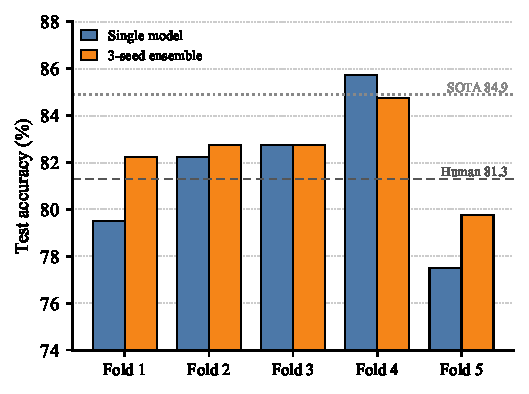
\includegraphics[width=0.80\columnwidth]{fig_folds.pdf}}
\caption{Per-fold test accuracy of the single FRESCA-Net (200-epoch, three-crop test-time augmentation) and the three-seed ensemble (300-epoch, seven-crop). Reference lines: human accuracy (81.3) and from-scratch state of the art (84.9). The ensemble mainly rescues the two weakest folds.}
\label{fig:folds}
\end{figure}

\subsection{Discussion and Limitations}
Three observations stand out. First, on a small, hard, from-scratch benchmark the architecture is the primary determinant of accuracy: the compact residual backbone with channel attention and a temporal-aware pooling head buys sixteen points over the classic baseline before any augmentation is added, whereas the augmentation adds under three. Modern design choices matter chiefly by making a small network optimise stably from little data rather than by adding raw representational power. Second, among the augmentations it is the energy-domain Between-Class mixing, applied in the waveform domain so that its energy-additive semantics stay exact, that keeps paying on top of a strong backbone \cite{tokozume_bc}. Third, the bottleneck is the data, not the capacity: the 300-epoch over-training result and the fold-to-fold variance both point to the sixteen-hundred-clip regime as the ceiling, so the productive direction is more effective data --- offline pitch-shifting and time-stretching to enlarge each fold, and more seeds to reduce variance --- rather than a deeper network.

A few limitations remain. The study is confined by design to the from-scratch, no-external-data setting, so the pretrained transformers that dominate the absolute leaderboard are cited only for orientation. All numbers come from a single shared recipe that isolates each factor at one fixed cost but does not show any model at its own optimum, and per-architecture tuning could move the absolute figures. Finally, a full per-class confusion study across seeds and a confirmation of the on-device latency that the compact size promises are natural next steps.

\section{Conclusion}
We presented FRESCA-Net, a compact 2.88 million-parameter convolutional network trained entirely from scratch on ESC-50 and evaluated under a single leakage-free five-fold protocol. Its frequency-aware squeeze-and-excitation backbone, anisotropic downsampling, attentive-statistics pooling and energy-domain Between-Class augmentation reach 81.55 percent as a single model and 82.45 percent as a three-seed ensemble, exceeding human accuracy and matching EnvNet-v2 with Between-Class learning without any external data. A matched ablation attributes the bulk of the accuracy to the architecture ($+16.45$ points) over the augmentation ($+2.90$), and the per-fold study exposes the small-data regime, not model capacity, as the ceiling. The work offers a reproducible reference for compact, from-scratch environmental sound recognition and a clean protocol on which future data-centric gains can be measured.

\begin{thebibliography}{00}
\bibitem{piczak_dataset} K. J. Piczak, ``ESC: Dataset for environmental sound classification,'' in \textit{Proc. 23rd ACM Int. Conf. Multimedia (MM)}, Brisbane, Australia, 2015, pp. 1015--1018, doi: 10.1145/2733373.2806390.
\bibitem{piczak_cnn} K. J. Piczak, ``Environmental sound classification with convolutional neural networks,'' in \textit{Proc. IEEE 25th Int. Workshop Mach. Learn. Signal Process. (MLSP)}, Boston, MA, USA, 2015, pp. 1--6, doi: 10.1109/MLSP.2015.7324337.
\bibitem{salamon_bello} J. Salamon and J. P. Bello, ``Deep convolutional neural networks and data augmentation for environmental sound classification,'' \textit{IEEE Signal Process. Lett.}, vol. 24, no. 3, pp. 279--283, 2017, doi: 10.1109/LSP.2017.2657381.
\bibitem{tokozume_envnet} Y. Tokozume and T. Harada, ``Learning environmental sounds with end-to-end convolutional neural network,'' in \textit{Proc. IEEE Int. Conf. Acoust., Speech, Signal Process. (ICASSP)}, New Orleans, LA, USA, 2017, pp. 2721--2725, doi: 10.1109/ICASSP.2017.7952651.
\bibitem{dai_rawwaveform} W. Dai, C. Dai, S. Qu, J. Li, and S. Das, ``Very deep convolutional neural networks for raw waveforms,'' in \textit{Proc. IEEE Int. Conf. Acoust., Speech, Signal Process. (ICASSP)}, 2017, pp. 421--425, doi: 10.1109/ICASSP.2017.7952190.
\bibitem{huzaifah_tf} M. Huzaifah, ``Comparison of time-frequency representations for environmental sound classification using convolutional neural networks,'' arXiv preprint arXiv:1706.07156, 2017.
\bibitem{tokozume_bc} Y. Tokozume, Y. Ushiku, and T. Harada, ``Learning from between-class examples for deep sound recognition,'' in \textit{Proc. Int. Conf. Learn. Represent. (ICLR)}, 2018, arXiv:1711.10282.
\bibitem{zhu_multiscale} B. Zhu, C. Wang, F. Liu, J. Lei, Z. Lu, and Y. Peng, ``Learning environmental sounds with multi-scale convolutional neural network,'' in \textit{Proc. Int. Joint Conf. Neural Netw. (IJCNN)}, Rio de Janeiro, Brazil, 2018, pp. 1--8, doi: 10.1109/IJCNN.2018.8489641.
\bibitem{aytar_soundnet} Y. Aytar, C. Vondrick, and A. Torralba, ``SoundNet: Learning sound representations from unlabeled video,'' in \textit{Advances in Neural Information Processing Systems (NeurIPS)}, vol. 29, 2016, pp. 892--900, arXiv:1610.09001.
\bibitem{hershey_cnnaudio} S. Hershey \textit{et al.}, ``CNN architectures for large-scale audio classification,'' in \textit{Proc. IEEE Int. Conf. Acoust., Speech, Signal Process. (ICASSP)}, New Orleans, LA, USA, 2017, pp. 131--135, doi: 10.1109/ICASSP.2017.7952132.
\bibitem{gemmeke_audioset} J. F. Gemmeke, D. P. W. Ellis, D. Freedman, A. Jansen, W. Lawrence, R. C. Moore, M. Plakal, and M. Ritter, ``Audio Set: An ontology and human-labeled dataset for audio events,'' in \textit{Proc. IEEE Int. Conf. Acoust., Speech, Signal Process. (ICASSP)}, New Orleans, LA, USA, 2017, pp. 776--780, doi: 10.1109/ICASSP.2017.7952261.
\bibitem{kong_panns} Q. Kong, Y. Cao, T. Iqbal, Y. Wang, W. Wang, and M. D. Plumbley, ``PANNs: Large-scale pretrained audio neural networks for audio pattern recognition,'' \textit{IEEE/ACM Trans. Audio, Speech, Language Process.}, vol. 28, pp. 2880--2894, 2020, doi: 10.1109/TASLP.2020.3030497.
\bibitem{gong_ast} Y. Gong, Y.-A. Chung, and J. Glass, ``AST: Audio spectrogram transformer,'' in \textit{Proc. Interspeech 2021}, 2021, pp. 571--575, doi: 10.21437/Interspeech.2021-698.
\bibitem{chen_beats} S. Chen, Y. Wu, C. Wang, S. Liu, D. Tompkins, Z. Chen, W. Che, X. Yu, and F. Wei, ``BEATs: Audio pre-training with acoustic tokenizers,'' in \textit{Proc. 40th Int. Conf. Mach. Learn. (ICML)}, PMLR vol. 202, 2023, pp. 5178--5193.
\bibitem{elizalde_clap} B. Elizalde, S. Deshmukh, M. Al Ismail, and H. Wang, ``CLAP: Learning audio concepts from natural language supervision,'' in \textit{Proc. IEEE Int. Conf. Acoust., Speech, Signal Process. (ICASSP)}, Rhodes Island, Greece, 2023, doi: 10.1109/ICASSP49357.2023.10095889.
\bibitem{guzhov_esresnet} A. Guzhov, F. Raue, J. Hees, and A. Dengel, ``ESResNet: Environmental sound classification based on visual domain models,'' in \textit{Proc. 25th Int. Conf. Pattern Recognit. (ICPR)}, 2021, pp. 4933--4940, doi: 10.1109/ICPR48806.2021.9413035.
\bibitem{palanisamy_rethinking} K. Palanisamy, D. Singhania, and A. Yao, ``Rethinking CNN models for audio classification,'' arXiv preprint arXiv:2007.11154, 2020.
\bibitem{izmailov_swa} P. Izmailov, D. Podoprikhin, T. Garipov, D. Vetrov, and A. G. Wilson, ``Averaging weights leads to wider optima and better generalization,'' in \textit{Proc. 34th Conf. Uncertainty in Artificial Intelligence (UAI)}, 2018, pp. 876--885, arXiv:1803.05407.
\bibitem{liu_coordconv} R. Liu, J. Lehman, P. Molino, F. P. Such, E. Frank, A. Sergeev, and J. Yosinski, ``An intriguing failing of convolutional neural networks and the CoordConv solution,'' in \textit{Proc. 32nd Int. Conf. Neural Inf. Process. Syst. (NeurIPS)}, 2018, pp. 9628--9639, arXiv:1807.03247.
\bibitem{park_specaugment} D. S. Park, W. Chan, Y. Zhang, C.-C. Chiu, B. Zoph, E. D. Cubuk, and Q. V. Le, ``SpecAugment: A simple data augmentation method for automatic speech recognition,'' in \textit{Proc. Interspeech 2019}, 2019, pp. 2613--2617, doi: 10.21437/Interspeech.2019-2680.
\bibitem{zhang_mixup} H. Zhang, M. Cisse, Y. N. Dauphin, and D. Lopez-Paz, ``mixup: Beyond empirical risk minimization,'' in \textit{Proc. Int. Conf. Learn. Represent. (ICLR)}, 2018, arXiv:1710.09412.
\bibitem{muller_labelsmoothing} R. M\"uller, S. Kornblith, and G. E. Hinton, ``When does label smoothing help?,'' in \textit{Proc. Adv. Neural Inf. Process. Syst. (NeurIPS)}, 2019, pp. 4694--4703, arXiv:1906.02629.
\bibitem{he_resnet} K. He, X. Zhang, S. Ren, and J. Sun, ``Deep residual learning for image recognition,'' in \textit{Proc. IEEE Conf. Comput. Vis. Pattern Recognit. (CVPR)}, Las Vegas, NV, USA, 2016, pp. 770--778, doi: 10.1109/CVPR.2016.90.
\bibitem{hu_senet} J. Hu, L. Shen, and G. Sun, ``Squeeze-and-excitation networks,'' in \textit{Proc. IEEE Conf. Comput. Vis. Pattern Recognit. (CVPR)}, Salt Lake City, UT, USA, 2018, pp. 7132--7141, doi: 10.1109/CVPR.2018.00745.
\bibitem{huang_stochastic} G. Huang, Y. Sun, Z. Liu, D. Sedra, and K. Q. Weinberger, ``Deep networks with stochastic depth,'' in \textit{Proc. Eur. Conf. Comput. Vis. (ECCV)}, 2016, pp. 646--661, doi: 10.1007/978-3-319-46493-0\_39.
\bibitem{okabe_asp} K. Okabe, T. Koshinaka, and K. Shinoda, ``Attentive statistics pooling for deep speaker embedding,'' in \textit{Proc. Interspeech 2018}, 2018, pp. 2252--2256, doi: 10.21437/Interspeech.2018-993.
\bibitem{kim_bcresnet} B. Kim, S. Chang, J. Lee, and D. Sung, ``Broadcasted residual learning for efficient keyword spotting,'' in \textit{Proc. Interspeech 2021}, 2021, pp. 4538--4542, doi: 10.21437/Interspeech.2021-383.
\bibitem{loshchilov_adamw} I. Loshchilov and F. Hutter, ``Decoupled weight decay regularization,'' in \textit{Proc. Int. Conf. Learn. Represent. (ICLR)}, New Orleans, LA, USA, 2019, arXiv:1711.05101.
\bibitem{loshchilov_sgdr} I. Loshchilov and F. Hutter, ``SGDR: Stochastic gradient descent with warm restarts,'' in \textit{Proc. Int. Conf. Learn. Represent. (ICLR)}, 2017, arXiv:1608.03983.
\bibitem{ioffe_bn} S. Ioffe and C. Szegedy, ``Batch normalization: accelerating deep network training by reducing internal covariate shift,'' in \textit{Proc. 32nd Int. Conf. Mach. Learn. (ICML)}, PMLR vol. 37, 2015, pp. 448--456, arXiv:1502.03167.
\end{thebibliography}

\end{document}
